\documentclass{article}
% Change "article" to "report" to get rid of page number on title page
\usepackage{amsmath,amsfonts,amsthm,amssymb}

\usepackage{ulem}
\usepackage{framed}
\usepackage{setspace}
\usepackage{Tabbing}
\usepackage{fancyhdr}
\usepackage{lastpage}
\usepackage{extramarks}
\usepackage{chngpage}
\usepackage{soul,color}
\usepackage{graphicx,float,wrapfig}
\usepackage{relsize}
\usepackage{tikz}

\graphicspath{ {c:/user/images/} }
\usepackage[rightcaption]{sidecap}


% In case you need to adjust margins:
\topmargin=-0.45in      %
\evensidemargin=0in     %
\oddsidemargin=0in      %
\textwidth=6.5in        %
\textheight=9.0in       %
\headsep=0.25in         %

\newcommand{\hmwkClass}{Lowering The Frequency Of Mass Shootings By Increasing Ammunition Taxes: A Mathematical Approach}

\newcommand{\hmwkAuthorName}{Warren\ Wilson}

% Setup the header and footer
\pagestyle{fancy}                                                       %
\lhead{\hmwkAuthorName}                                                 %
\chead{\hmwkClass\ - \hmwkTitle}  %
\rhead{\firstxmark}                                                     %
\lfoot{\lastxmark}                                                      %
\cfoot{}                                                                %
\rfoot{Page\ \thepage\ of\ \pageref{LastPage}}                          %
\renewcommand\headrulewidth{0.4pt}                                      %
\renewcommand\footrulewidth{0.4pt}                                      %
\newcommand{\enterProblemHeader}[1]{\nobreak\extramarks{#1}{#1 continued on next page\ldots}\nobreak%
                                    \nobreak\extramarks{#1 (continued)}{#1 continued on next page\ldots}\nobreak}%
\newcommand{\exitProblemHeader}[1]{\nobreak\extramarks{#1 (continued)}{#1 continued on next page\ldots}\nobreak%
                                   \nobreak\extramarks{#1}{}\nobreak}%

\newlength{\labelLength}
\newcommand{\labelAnswer}[2]
  {\settowidth{\labelLength}{#1}%
   \addtolength{\labelLength}{0.25in}%
   \changetext{}{-\labelLength}{}{}{}%
   \noindent\fbox{\begin{minipage}[c]{\columnwidth}#2\end{minipage}}%
   \marginpar{\fbox{#1}}%

   % We put the blank space above in order to make sure this
   % \marginpar gets correctly placed.
   \changetext{}{+\labelLength}{}{}{}}%

\setcounter{secnumdepth}{0}
\newcommand{\homeworkProblemName}{}%
\newcounter{homeworkProblemCounter}%
\newenvironment{homeworkProblem}[1][Problem \arabic{homeworkProblemCounter}]%
  {\stepcounter{homeworkProblemCounter}%
   \renewcommand{\homeworkProblemName}{#1}%
   \section{\homeworkProblemName}%
   \enterProblemHeader{\homeworkProblemName}}%
  {\exitProblemHeader{\homeworkProblemName}}%

\newcommand{\problemAnswer}[1]
  {\noindent\fbox{\begin{minipage}[c]{\columnwidth}#1\end{minipage}}}%

\newcommand{\problemLAnswer}[1]
  {\labelAnswer{\homeworkProblemName}{#1}}

\newcommand{\homeworkSectionName}{}%
\newlength{\homeworkSectionLabelLength}{}%
\newenvironment{homeworkSection}[1]%
  {% We put this space here to make sure we're not connected to the above.
   % Otherwise the changetext can do funny things to the other margin

   \renewcommand{\homeworkSectionName}{#1}%
   %\settowidth{\homeworkSectionLabelLength}{\homeworkSectionName}%
   %\addtolength{\homeworkSectionLabelLength}{0in}%
   \changetext{}{-\homeworkSectionLabelLength}{}{}{}%
   \subsection{\homeworkSectionName}%
   \enterProblemHeader{\homeworkProblemName\ [\homeworkSectionName]}}%
  {\enterProblemHeader{\homeworkProblemName}%

   % We put the blank space above in order to make sure this margin
   % change doesn't happen too soon (otherwise \sectionAnswer's can
   % get ugly about their \marginpar placement.
   \changetext{}{+\homeworkSectionLabelLength}{}{}{}}%

\newcommand{\sectionAnswer}[1]
  {% We put this space here to make sure we're disconnected from the previous
   % passage

   \noindent\fbox{\begin{minipage}[c]{\columnwidth}#1\end{minipage}}%
   \enterProblemHeader{\homeworkProblemName}\exitProblemHeader{\homeworkProblemName}%
   %\marginpar{\fbox{\homeworkSectionName}}%

   % We put the blank space above in order to make sure this
   % \marginpar gets correctly placed.
   }%

%%%%%%%%%%%%%%%%%%%%%%%%%%%%%%%%%%%%%%%%%%%%%%%%%%%%%%%%%%%%%


%%%%%%%%%%%%%%%%%%%%%%%%%%%%%%%%%%%%%%%%%%%%%%%%%%%%%%%%%%%%% 
% Make title
\title{\vspace{2in}\textmd{\textbf{\hmwkClass\ \hmwkTitle}}\\\normalsize\vspace{0.1in}\small{ \hmwkDueDate}\\\vspace{0.1in}\large{\textit{\hmwkClassInstructor\ \hmwkClassTime}}\vspace{3in}}
\date{}
\author{\textbf{\hmwkAuthorName}}
%%%%%%%%%%%%%%%%%%%%%%%%%%%%%%%%%%%%%%%%%%%%%%%%%%%%%%%%%%%%%

\begin{document}
\begin{spacing}{1.1}
\maketitle
\newpage

\tableofcontents
\newpage

% When problems are long, it may be desirable to put a \newpage or a
% \clearpage before each homeworkProblem environment

\newpage
\begin{homeworkProblem}[Pre-Amble]
    
    In the USA, from as early as 1949, mass shootings have always been a source of many heated political debates. Not least of which, is how as a nation are we to punish mass shooters, but instead, how do we as a nation plan to ensure that mass shootings do not become commonplace?\\\\
    As it currently stands, the two most common arguments are that: unrestricted gun availability promotes the occurrence of firearm-induced homicides or, that gun possession can protect potential victims when attacked.\\\\
    In the words of the late New York senator Daniel Patrick Moynihan, "Guns don't kill people; bullets do...It is time the Federal Government began taxing handgun ammunition used in crime out of existence"[1]. While on its face, the idea of increasing the tax on ammunition might seem novel, this notion has seen its fair share of attention on the senate floor.\\\\
    In 1993 the New York Times reported on Senator Daniel Patrick Moynihan, saying that he would insist that President Clinton's health-care plan include a huge increase in Federal taxes on handgun ammunition that would make some especially destructive bullets unaffordable.\\\\
    As one would imagine, this idea was simply disregarded as being quixotic. But seeing that this is coming from the chairman of the Finance Committee, one of the two Senate committees with a predominant role on the health bill, a proposal to tax ammunition immediately becomes a serious issue [1].\\\\
    The purpose of this paper is to provide a mathematical analysis of NY senator Moynihan's potential third solution.
   
\end{homeworkProblem}
\newpage
\begin{homeworkProblem}[Terminology]
    \begin{homeworkSection}{Rounds}
The term "round" refers to a single piece of ammunition. This may mean a single metallic cartridge with its casing and bullet, a shotgun shell casing and its pellets or slug, or a muzzleloader powder load and projectile. The term should not be confused with the bullet, which is the metal projectile that is accelerating off the metal cartridge casing, through the gun barrel and downrange when the trigger is pulled. The bullet itself actually ceases to be "round" as soon as it accelerates down the gun barrel.[2]    
\end{homeworkSection}
\begin{homeworkSection}{Caliber}
In guns, particularly firearms, caliber or calibre is the approximate internal diameter of the gun barrel, or the diameter of the projectile it shoots. It is measured in hundredths or thousandths of an inch or in millimetres. For example, a ".45 caliber" firearm has a barrel diameter of roughly 0.45 inches (11 mm). Barrel diameters can also be expressed using metric dimensions. For example, a "9mm pistol" has a barrel diameter of about 9 millimetres (it is rare for the actual barrel diameter to precisely match the designation however, and the bullet itself is yet another dimension). When the barrel diameter is given in inches, the abbreviation "cal" (for "caliber") can be used. For example, a small-bore rifle with a diameter of 0.22 inches (5.6 mm) can be referred to as ".22" or a ".22 cal"; however, the decimal point is generally dropped when spoken, making it a "twenty-two" or a "two-two caliber", or a ".45 caliber" would be a "forty-five", or "forty-five caliber", etc.[3]
    \end{homeworkSection}
    \begin{homeworkSection}{Assault Rifle}
To start, AR does NOT stand for “Assault Rifle”. The “AR” comes from the firearms manufacturer Armalite. Those letters are used as a standard naming practice for their firearms. Just like the Ford F-150, the AR-15 is just a specific model. So what is an Assault Rifle? Is an AR-15 an assault rifle? An assault rifle is a rifle that: has selectable firing modes, and can fire in fully automatic mode. Select fire means that there is a switch to toggle between firing modes. AR-15's do not fit this definition, therefore they are not assault rifles.[4]
    \end{homeworkSection}
    \begin{homeworkSection}{Semi-Automatic}
Semiautomatic means that when the trigger is pulled, the following happens: a bullet is fired,
the spent bullet casing is ejected from the firearm, and the next bullet round is loaded into the firing chamber. One trigger pull $=$ one bullet fired. That is how most handguns work, how many rifles work and even how some shotguns work. Pull the trigger and one bullet comes out. Just one and only one. A firearm that fires one bullet at a time and loads the next round into the chamber is called a “semiautomatic” firearm. Semiautomatic rifles are NOT assault rifles.

There is another firing mode that is called “fully automatic”. In the case of full auto firearms, when the trigger is pulled and held down, the firearm will shoot continuously until the trigger is released or until the gun runs out of ammunition. A fully automatic firearm is often referred to as a “machine gun”. Machine guns can be described as assault rifles.[4]
\end{homeworkSection}
    \begin{homeworkSection}{Mass Shooting}
 According to CNN, a mass shooting is defined as having four or more fatalities, not including gang killings or slayings that involve the death of multiple family members.[5]
    \end{homeworkSection}
\end{homeworkProblem}


\newpage
\begin{homeworkProblem}[The Modelling Approach]
    \begin{homeworkSection}{Rationale}
        The rational for this model is as follows:  We began by asking ourselves, "would increasing the tax on ammunition lead to a decrease in the frequency of mass shootings?". This question immediately gives rise to the following question, "if implemented, who are the people that will be most affected?" Or tangentially, "do rich people commit mass shootings? Do poor homeless people commit mass shootings? If so, what is the frequency?". With these questions in place, we first set out to address the question that underpins this entire model, "what is the general socioeconomic demographic of mass shooters?" 
    \end{homeworkSection}
    \begin{homeworkSection}{Solution}
        We focused on the 32 most deadly mass shootings (ranging from 8-58 fatalities per shooting) in American history, and then proceeded to compile data about the shooters. The following graphs were generated:\\
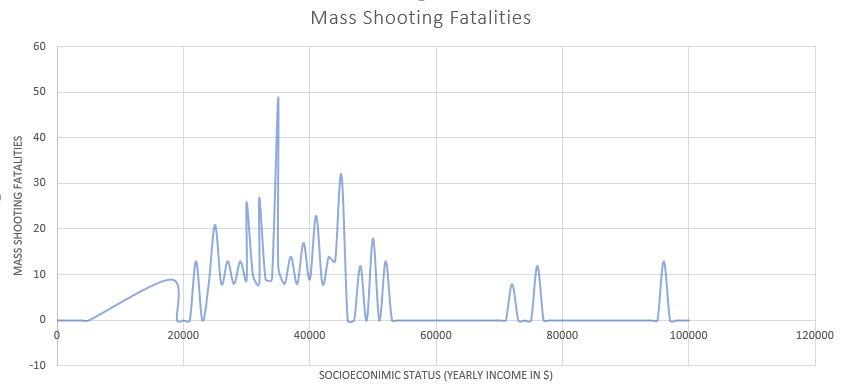
\includegraphics[width=16.5cm, height=6cm]{mass1}\\
Based on this visual, it becomes apparent that there is a higher concentration of fatalities when the shooters are from the lower class to lower middle class (\$16,000-\$47,000). It is worth pointing out that there was one outlier, in the case of the Las Vegas shooter who was in the rich class (\$1,000,000 and above) and killed 58 people, as shown in the graphic below:\\
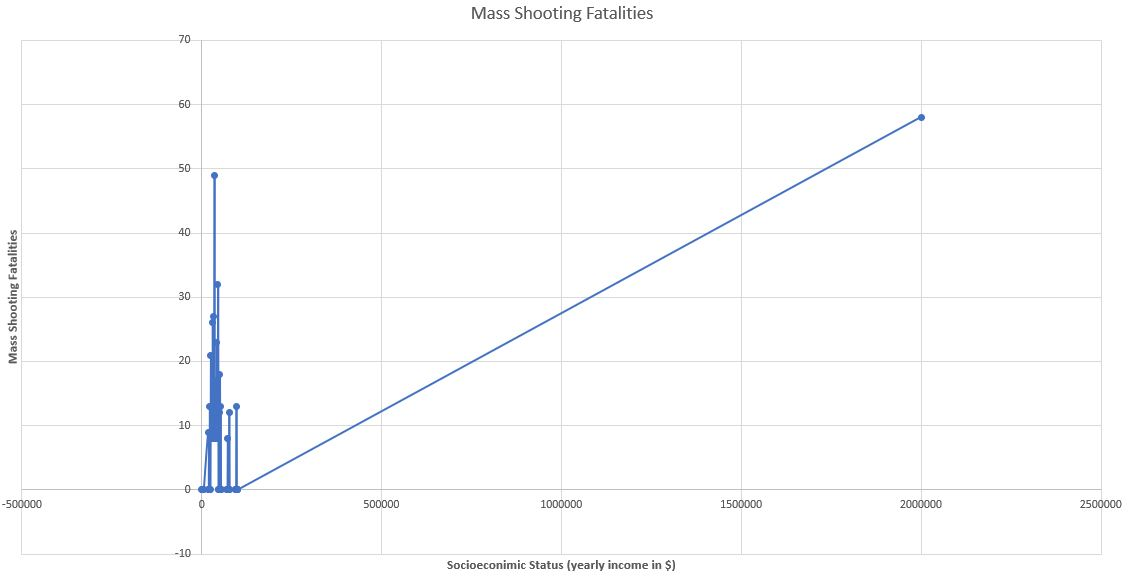
\includegraphics[width=16.5cm, height=8cm]{mass2}\\
Based on our rational we begun to assign a few parameters:\\
Tax $=\tau$\\
Number of ammunition sold $=\alpha$\\
Adjusted cost for ammunition $=\alpha+\alpha\tau$\\
Cost of guns $=g$\\
Mass shooting fatalities $=m$\\
Socioeconomic status of the shooter $=x$\\
Yearly ammunition sales $=S$\\
From this, we let $S(\tau)=$ yearly ammunition sales (in units) as a function of tax.\\
\\
The next task is to investigate the relationship of how taxation affects consumer behavior based on existing market research for similarly priced items. One potential approach might be to think of this model in terms of a variation of the Sigmoid function (logistic), perhaps a model that behaves something like: $$\displaystyle{\frac{d\alpha}{d\tau}=\frac{-2\alpha}{e^{-\tau}+1}}$$\\
\\
Due to the difficult/expensive nature of gathering meaningful market data (trends, tax data, sales figures in units or dollars), certain key assumptions were made. As a result of these assumptions, this model will be a provisional one, and will therefore need to be updated as new information arises.\\
\\
\textbf{Assumptions:}
\begin{itemize}
  \item Approximately $90$ billion rounds of ammunition were sold during President Barack Obama's presidency. (This number was determined by dividing the estimated 17 billion dollars spent on ammunition during President Obama's presidency by the average cost of (0.19cents) a single round of ammunition). This number will serve as the amount of ammunition sold when no new tax imposition.
  \item The choice in using a variation of the Sigmoid function (which is a special case of the logistic function) is because the Sigmoid function is one of the most widely utilized functions in business optimization, in addition to its general shape making the most intuitive sense. The Sigmoid curve is an algebraic function which suggests that no growth is permanent, or sustainable forever and that every growth curve will eventually hit a plateau, and if not addressed, that plateau will turn into the decline of the business.Therefore it was reasonable to assume that this modified function should behave like what would happen to a company's sales if they inappropriately priced (too high) their goods.
  \item Given the estimated 90 billion rounds of ammunition sold during President Barack Obama's presidency, if it were possible to look at what percentage of ammunition sold was purchased by people making between \$16,000 and \$47,000, we could then place a horizontal line at the amount of ammunition sold to that demographic, then wherever the function crosses that line would be at the tax needed to reduce the number of rounds of ammunition sold within that demographic. Because such information is not forthcoming, an arbitrary horizontal line was constructed and was assumed to be 42 billion.
\end{itemize}
\newpage
\textbf{VISUAL AID}\\
$$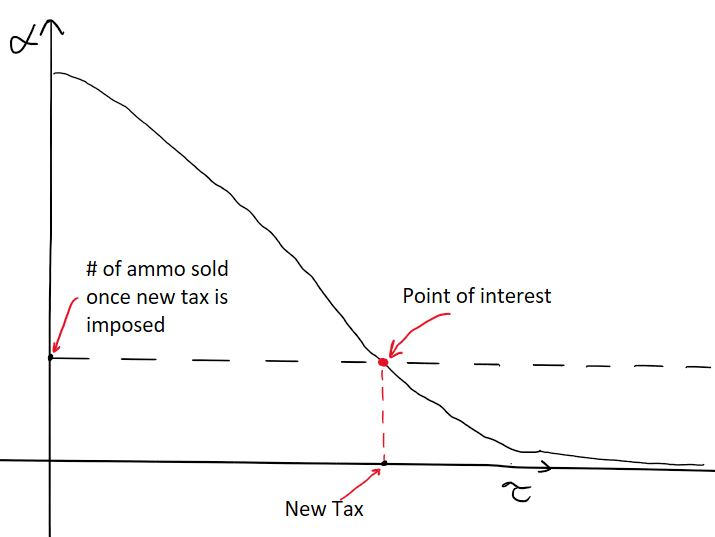
\includegraphics[width=13.5cm, height=6cm]{gunCapture}$$\\

\textbf{Calculations}: 
$$\displaystyle{\frac{d\alpha(\tau)}{d\tau}=\frac{-2\alpha(\tau)}{e^{-\tau}+1}}$$
$$\displaystyle{\int\frac{-1}{2\alpha}d\alpha=\int\frac{1}{e^\tau+1}d\tau}$$
$$\bigg(\frac{-1}{2}\bigg)ln(\alpha)=ln(e^{\tau}+1)+c$$
$$\frac{1}{\sqrt{e^{ln\alpha}}}=e^{ln(e^\tau+1)}e^c$$
$$\frac{1}{\sqrt{\alpha}}=(e^\tau+1)k$$\\
With the initial conditions $(\tau_0,\alpha_0)=(0,90\times10^9)$ we have,
$$\tau=0\rightarrow{2k}=\frac{1}{\sqrt{90\times10^9}}$$
$$\boxed{k=\frac{1}{2\sqrt{90\times10^9}}}$$
$$\frac{1}{\sqrt{\alpha}}=\frac{(e^\tau+1)}{2\sqrt{90\times10^9}}$$\\
Therefore the function that models ammunition sales in units with respect to tax is given by:\\
$$\boxed{\alpha(\tau)=\Bigg(\frac{(e^\tau+1)}{2\sqrt{90\times10^9}}\Bigg)^{-2}}$$\\

\newpage
Plotting $\alpha(\tau)=\Bigg(\displaystyle{\frac{(e^\tau+1)}{2\sqrt{90\times10^9}}}\Bigg)^{-2}$ and $\alpha(\tau)=42\times10^9$ on the same graph gives the point of intersection associated with the new tax that will reduce ammunition unit sales down to $42\times10^9$.
$$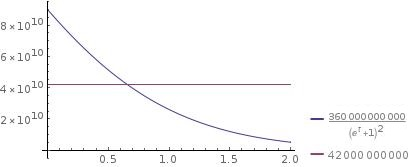
\includegraphics[width=9.8cm, height=4cm]{WolframAlphaplot}$$\\
The point of intersection occurs $\tau=0.6563$, which corresponds to a  $65.63\%$ tax increase. \\\\
While this result gives us a fairly high tax increase, it serves as a reasonable starting point for which a more in depth market analysis can be conducted. As access to more information becomes possible, this model will be updated to reflect that information.




\end{homeworkSection}
\end{homeworkProblem}
\newpage
\begin{homeworkProblem}[Works Cited]

\ \ \ \ [1] Moynihan Asks Big Tax Increase On Ammunition\\
https://www.nytimes.com/1993/11/04/us/moynihan-asks-big-tax-increase-on-ammunition.html\\
\\

[2] A Definition of the Term "Round" in Firearm Shooting\\
https://www.thoughtco.com/definition-of-round-ammunition-ammo-skeet-1926820\\
\\

[3] Caliber\\
https://en.wikipedia.org/wiki/Caliber\\
\\

[4] What is and is NOT an Assault Rifle\\
http://www.thefirearms.guide/blog/educational/assault-rifle\\
\\

[5] Mass shooting\\
https://en.wikipedia.org/wiki/Mass_shooting#Definition\\
\\

[6] US Mass Shootings, 1982-2018: Data From Mother Jones’ Investigation\\
https://www.motherjones.com/politics/2012/12/mass-shootings-mother-jones-full-data/\\

[7] Deadliest Mass Shootings in Modern US History Fast Facts\\
https://www.cnn.com/2013/09/16/us/20-deadliest-mass-shootings-in-u-s-history-fast-facts/index.htm\\
\\

[8] https://www.washingtonpost.com/news/politics/wp/2017/03/22/americans-spent-an-estimated-17-billion-dollars-on-ammunition-while-obama-was-president/?utm_term=.5bed4c67a116

\end{homeworkProblem}
\end{spacing}
\end{document}
